\documentclass{ximera}

%\usepackage{todonotes}

\newcommand{\todo}{}

\usepackage{tkz-euclide}
\tikzset{>=stealth} %% cool arrow head
\tikzset{shorten <>/.style={ shorten >=#1, shorten <=#1 } } %% allows shorter vectors

\usepackage{tkz-tab}  %% sign charts
\usetikzlibrary{decorations.pathreplacing} 

\usetikzlibrary{backgrounds} %% for boxes around graphs
\usetikzlibrary{shapes,positioning}  %% Clouds and stars
\usetikzlibrary{matrix} %% for matrix
\usepgfplotslibrary{polar} %% for polar plots
\usetkzobj{all}
\usepackage[makeroom]{cancel} %% for strike outs
%\usepackage{mathtools} %% for pretty underbrace % Breaks Ximera
\usepackage{multicol}

\usepackage{polynom}



\usepackage[many]{tcolorbox}  %% for titled boxes
\newtcolorbox{xbox}[1]{%
    tikznode boxed title,
    enhanced,
    arc=0mm,
    interior style={white},
    attach boxed title to top center= {yshift=-\tcboxedtitleheight/2},
    fonttitle=\bfseries,
    colbacktitle=white,coltitle=black,
    boxed title style={size=normal,colframe=white,boxrule=0pt},
    title={#1}}


\usepackage{array}
\setlength{\extrarowheight}{+.1cm}   
\newdimen\digitwidth
\settowidth\digitwidth{9}
\def\divrule#1#2{
\noalign{\moveright#1\digitwidth
\vbox{\hrule width#2\digitwidth}}}





\newcommand{\RR}{\mathbb R}
\newcommand{\R}{\mathbb R}
\newcommand{\N}{\mathbb N}
\newcommand{\Z}{\mathbb Z}

%\renewcommand{\d}{\,d\!}
\renewcommand{\d}{\mathop{}\!d}
\newcommand{\dd}[2][]{\frac{\d #1}{\d #2}}
\newcommand{\pp}[2][]{\frac{\partial #1}{\partial #2}}
\renewcommand{\l}{\ell}
\newcommand{\ddx}{\frac{d}{\d x}}
\newcommand{\ddt}{\frac{d}{\d t}}

\newcommand{\zeroOverZero}{\ensuremath{\boldsymbol{\tfrac{0}{0}}}}
\newcommand{\inftyOverInfty}{\ensuremath{\boldsymbol{\tfrac{\infty}{\infty}}}}
\newcommand{\zeroOverInfty}{\ensuremath{\boldsymbol{\tfrac{0}{\infty}}}}
\newcommand{\zeroTimesInfty}{\ensuremath{\small\boldsymbol{0\cdot \infty}}}
\newcommand{\inftyMinusInfty}{\ensuremath{\small\boldsymbol{\infty - \infty}}}
\newcommand{\oneToInfty}{\ensuremath{\boldsymbol{1^\infty}}}
\newcommand{\zeroToZero}{\ensuremath{\boldsymbol{0^0}}}
\newcommand{\inftyToZero}{\ensuremath{\boldsymbol{\infty^0}}}



\newcommand{\numOverZero}{\ensuremath{\boldsymbol{\tfrac{\#}{0}}}}
\newcommand{\dfn}{\textbf}
%\newcommand{\unit}{\,\mathrm}
\newcommand{\unit}{\mathop{}\!\mathrm}
\newcommand{\eval}[1]{\bigg[ #1 \bigg]}
\newcommand{\seq}[1]{\left( #1 \right)}
\renewcommand{\epsilon}{\varepsilon}
\renewcommand{\iff}{\Leftrightarrow}

\DeclareMathOperator{\arccot}{arccot}
\DeclareMathOperator{\arcsec}{arcsec}
\DeclareMathOperator{\arccsc}{arccsc}
\DeclareMathOperator{\si}{Si}
\DeclareMathOperator{\proj}{proj}
\DeclareMathOperator{\scal}{scal}


\newcommand{\tightoverset}[2]{% for arrow vec
  \mathop{#2}\limits^{\vbox to -.5ex{\kern-0.75ex\hbox{$#1$}\vss}}}
\newcommand{\arrowvec}[1]{\tightoverset{\scriptstyle\rightharpoonup}{#1}}
\renewcommand{\vec}{\mathbf}
\newcommand{\veci}{\vec{i}}
\newcommand{\vecj}{\vec{j}}
\newcommand{\veck}{\vec{k}}
\newcommand{\vecl}{\boldsymbol{\l}}

\newcommand{\dotp}{\bullet}
\newcommand{\cross}{\boldsymbol\times}
\newcommand{\grad}{\boldsymbol\nabla}
\newcommand{\divergence}{\grad\dotp}
\newcommand{\curl}{\grad\cross}
%\DeclareMathOperator{\divergence}{divergence}
%\DeclareMathOperator{\curl}[1]{\grad\cross #1}


\colorlet{textColor}{black} 
\colorlet{background}{white}
\colorlet{penColor}{blue!50!black} % Color of a curve in a plot
\colorlet{penColor2}{red!50!black}% Color of a curve in a plot
\colorlet{penColor3}{red!50!blue} % Color of a curve in a plot
\colorlet{penColor4}{green!50!black} % Color of a curve in a plot
\colorlet{penColor5}{orange!80!black} % Color of a curve in a plot
\colorlet{fill1}{penColor!20} % Color of fill in a plot
\colorlet{fill2}{penColor2!20} % Color of fill in a plot
\colorlet{fillp}{fill1} % Color of positive area
\colorlet{filln}{penColor2!20} % Color of negative area
\colorlet{fill3}{penColor3!20} % Fill
\colorlet{fill4}{penColor4!20} % Fill
\colorlet{fill5}{penColor5!20} % Fill
\colorlet{gridColor}{gray!50} % Color of grid in a plot

\newcommand{\surfaceColor}{violet}
\newcommand{\surfaceColorTwo}{redyellow}
\newcommand{\sliceColor}{greenyellow}




\pgfmathdeclarefunction{gauss}{2}{% gives gaussian
  \pgfmathparse{1/(#2*sqrt(2*pi))*exp(-((x-#1)^2)/(2*#2^2))}%
}


%%%%%%%%%%%%%
%% Vectors
%%%%%%%%%%%%%

%% Simple horiz vectors
\renewcommand{\vector}[1]{\left\langle #1\right\rangle}


%% %% Complex Horiz Vectors with angle brackets
%% \makeatletter
%% \renewcommand{\vector}[2][ , ]{\left\langle%
%%   \def\nextitem{\def\nextitem{#1}}%
%%   \@for \el:=#2\do{\nextitem\el}\right\rangle%
%% }
%% \makeatother

%% %% Vertical Vectors
%% \def\vector#1{\begin{bmatrix}\vecListA#1,,\end{bmatrix}}
%% \def\vecListA#1,{\if,#1,\else #1\cr \expandafter \vecListA \fi}

%%%%%%%%%%%%%
%% End of vectors
%%%%%%%%%%%%%

%\newcommand{\fullwidth}{}
%\newcommand{\normalwidth}{}



%% makes a snazzy t-chart for evaluating functions
%\newenvironment{tchart}{\rowcolors{2}{}{background!90!textColor}\array}{\endarray}

%%This is to help with formatting on future title pages.
\newenvironment{sectionOutcomes}{}{} 



%% Flowchart stuff
%\tikzstyle{startstop} = [rectangle, rounded corners, minimum width=3cm, minimum height=1cm,text centered, draw=black]
%\tikzstyle{question} = [rectangle, minimum width=3cm, minimum height=1cm, text centered, draw=black]
%\tikzstyle{decision} = [trapezium, trapezium left angle=70, trapezium right angle=110, minimum width=3cm, minimum height=1cm, text centered, draw=black]
%\tikzstyle{question} = [rectangle, rounded corners, minimum width=3cm, minimum height=1cm,text centered, draw=black]
%\tikzstyle{process} = [rectangle, minimum width=3cm, minimum height=1cm, text centered, draw=black]
%\tikzstyle{decision} = [trapezium, trapezium left angle=70, trapezium right angle=110, minimum width=3cm, minimum height=1cm, text centered, draw=black]


\outcome{Determine how the graph of a function looks without using a calculator.}

\title[Dig-In:]{Computations for graphing functions}

\begin{document}
\begin{abstract}
  We will give some general guidelines for sketching the plot of a
  function.
\end{abstract}
\maketitle

Let's get to the point. Here we use all of the tools we know to sketch
the graph of $y=f(x)$:


\begin{itemize}
\item Find the $y$-intercept, this is the point $(0,f(0))$. Place this
  point on your graph.
\item Find any vertical asymptotes, these are points $x=a$ where
  $f(x)$ goes to infinity as $x$ goes to $a$ (from the right, left, or
  both).
  \item If possible, find the $x$-intercepts, the points where $f(x) =
  0$. Place these points on your graph.
\item Analyze end behavior:  as $x \to \pm \infty$, what happens to the graph of $f$?  Does it  have horizontal asymptotes, increase or decrease without bound, or have some other kind of behavior?
\item Compute $f'$ and $f''$.
\item Find the critical points (the points where $f'(x) = 0$ or
  $f'(x)$ is undefined).
\item Use either the first or second derivative test to identify local extrema and/or
  find the intervals where your function is increasing/decreasing.
\item Find the candidates for inflection points, the points where
  $f''(x) = 0$ or $f''(x)$ is undefined.
\item Identify inflection points and concavity.

\item Determine an interval that shows all relevant behavior.
\end{itemize}
At this point you should be able to sketch the plot of your function.

\begin{example}
Sketch the graph of the function defined by $f(x)=2x^3-3x^2-12x$.

The $y$-intercept is $(0,\answer[given]{0})$. Place this point on your plot.
\begin{image}
\begin{tikzpicture}
	\begin{axis}[
            domain=-2:4,
            xmin=-2,
            xmax=4,
            ymax=25,
            ymin=-25,
            axis lines =middle, xlabel=$x$, ylabel=$y$,
            every axis y label/.style={at=(current axis.above origin),anchor=south},
            every axis x label/.style={at=(current axis.right of origin),anchor=west}
          ]
         \addplot[color=penColor,fill=penColor,only marks,mark=*] coordinates{(0,0)};  %% closed hole
        \end{axis}
\end{tikzpicture}
%% \caption{We start by placing the point $(0,0)$.}
%\label{figure:CS1}
\end{image}



Which of the following are vertical asymptotes?  Select all that apply.

\begin{selectAll}
	\choice{$x=0$}
	\choice{$x=1$}
	\choice{$x=-1$}
	\choice{$x=\sqrt{2}$}
	\choice[correct]{There are no vertical asymptotes}
\end{selectAll}

In this case, $f(x) =2x^3-3x^2-12x$, we can find the
$x$-intercepts.   There are three $x$ intercepts.  Call them $a$, $b$, and $c$, and order them such that $a<b<c$.  Then

\begin{align*}
  a &= \answer[given]{\frac{3-\sqrt{105}}{4}},\\
  b &= \answer[given]{0}, \\
  c &= \answer[given]{\frac{3+\sqrt{105}}{4}}.
\end{align*}


	
  Which of the following best describes the end behavior of $f$ as $x \to \infty$?		
  \begin{multipleChoice}
    \choice[correct]{$f$  increases without bound.}
    \choice{$f$ decreases without bound.}
    \choice{$f$ has a horizontal asymptote.}
    \choice{$f$ has some other behavior at $\infty$.}
  \end{multipleChoice}
  Which of the following best describes the end behavior of $f$ as $x \to -\infty$?		
  \begin{multipleChoice}
    \choice{$f$  increases without bound.}
    \choice[correct]{$f$ decreases without bound.}
    \choice{$f$ has a horizontal asymptote.}
    \choice{$f$ has some other behavior at $\infty$.}
  \end{multipleChoice}

Compute $f'(x)$ and $f''(x)$,
\[
f'(x) = \answer[given]{6x^2 -6x -12}=6(\answer{x^2-x-2})=6(x+1)(\answer{x-2}); \hspace{0.2in} f''(x) = \answer[given]{12x-6}=12(\answer{x-\frac{1}{2}}).
\]

The critical points are where $f'(x) = 0$, thus we need to solve $6(x+1)(x-2)
 = 0$ for $x$.   This equation has two solutions.  If we call them $a$ and $b$, with $a<b$, then what are $a$ and $b$?
\[
a = \answer[given]{-1}\qquad\text{and}\qquad b = \answer[given]{2}.
\]

Mark the critical points $x=2$ and $x=-1$ on your plot. %%BADBAD either or answer would be nice
\begin{image}
\begin{tikzpicture}
	\begin{axis}[
            domain=-2:4,
            xmin=-2,
            xmax=4,
            ymax=25,
            ymin=-25,
            axis lines =middle, xlabel=$x$, ylabel=$y$,
            every axis y label/.style={at=(current axis.above origin),anchor=south},
            every axis x label/.style={at=(current axis.right of origin),anchor=west}
          ]
         \addplot [dashed, penColor2] plot coordinates {(-1,-25) (-1,25)}; 
         \addplot [dashed, penColor2] plot coordinates {(2,-25) (2,25)}; 
         \addplot[color=penColor,fill=penColor,only marks,mark=*] coordinates{(0,0)};  %% closed hole
        \end{axis}
\end{tikzpicture}
%\caption{Now we add the critical points $x=-1$ and $x=2$.}
%\label{figure:CS2}
\end{image}
Since $f'(x)=6(x+1)(x-2)$, and both factors  $(x+1)$ and $(x-2)$ are negative for $x<-1$,  it follows that $f'(x)>0$, and , therefore, our  function is \wordChoice{\choice[correct]{increasing} \choice{decreasing}} on
$(-\infty,-1)$.\\
 Similarly, since for $-1<x<2$, $(x+1)>0$ and $ (x-2)<0$, the derivative is negative there, and , therefore, our function is \wordChoice{\choice{increasing} \choice[correct]{decreasing}} on $(-1,2)$.\\
  And, for $x>2$, both factors $(x+1)$ and $x-2)$ are positive, and , therefore, our function is  \wordChoice{\choice[correct]{increasing} \choice{decreasing}} on $(2,\infty)$. \\
  
Hence $x=-1$, corresponding to the point $(-1,7)$ is a local \wordChoice{\choice[correct]{maximum} \choice{minimum}}
and $x=2$, corresponding to the point $(2,-20)$ is local \wordChoice{\choice{maximum} \choice[correct]{minimum}} of
$f(x)$. Identify this on your plot.


\begin{image}
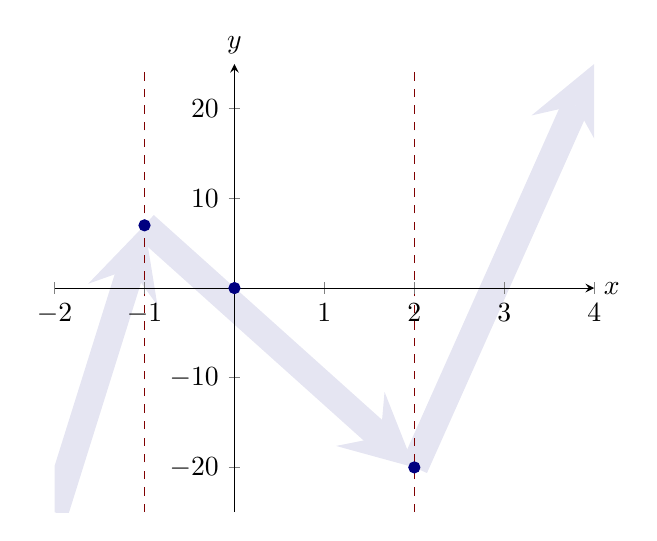
\begin{tikzpicture}
	\begin{axis}[
            axis on top=true,
            domain=-2:4,
            xmin=-2,
            xmax=4,
            ymax=25,
            ymin=-25,
            axis lines =middle, xlabel=$x$, ylabel=$y$,
            every axis y label/.style={at=(current axis.above origin),anchor=south},
            every axis x label/.style={at=(current axis.right of origin),anchor=west}
          ]
          \addplot [->, line width=10, penColor!10!background] plot coordinates {(-2,-25) (-1,7)}; 
          \addplot [->, line width=10, penColor!10!background] plot coordinates {(-1,7) (2,-20)}; 
          \addplot [->, line width=10, penColor!10!background] plot coordinates {(2,-20) (4,25)}; 
          \addplot [dashed, penColor2] plot coordinates {(-1,-25) (-1,25)}; 
          \addplot [dashed, penColor2] plot coordinates {(2,-25) (2,25)}; 
          \addplot [color=penColor,fill=penColor,only marks,mark=*] coordinates{(0,0)};  %% closed hole
          \addplot [color=penColor,fill=penColor,only marks,mark=*] coordinates{(-1,7)};  %% closed hole
          \addplot [color=penColor,fill=penColor,only marks,mark=*] coordinates{(2,-20)};  %% closed hole
          %\addplot [very thick, penColor, samples=100, smooth,domain=(-1.2:-.8)] {2*x^3-3*x^2-12*x};
          %\addplot [very thick, penColor, samples=100, smooth,domain=(1.8:2.2)] {2*x^3-3*x^2-12*x};
        \end{axis}
\end{tikzpicture}
%% \caption{We have identified the local extrema of $f(x)$ and where this
%%   function is increasing and decreasing.}
%% \label{figure:CS3}
\end{image}

The candidates for the inflection points are where $f''(x) = 0$, thus
we need to solve $12(x-\frac{1}{2})=0$ for $x$.  

The solution to this is $x = \answer{\frac{1}{2}}$.

This is only a \textbf{possible} inflection point, since the concavity needs to change to make it a true inflection point.\\

 We have that $f''(x)<0$ for $x<\frac{1}{2}$, therefore
$f$ is concave \wordChoice{\choice{up} \choice[correct]{down}}on $(-\infty,\frac{1}{2})$.\\

Similarly, $f''(x)>0$ for $x>\frac{1}{2}$, therefore
$f$ is concave \wordChoice{\choice[correct]{up} \choice{down}} on $(\frac{1}{2},\infty)$.

So this point \wordChoice{\choice[correct]{is} \choice{is not}} a point of inflection.

Since all of this behavior as described above occurs on the interval
$[-2,4]$, we now have a complete sketch of $f(x)$ on this interval,
see the figure below.
\begin{image}
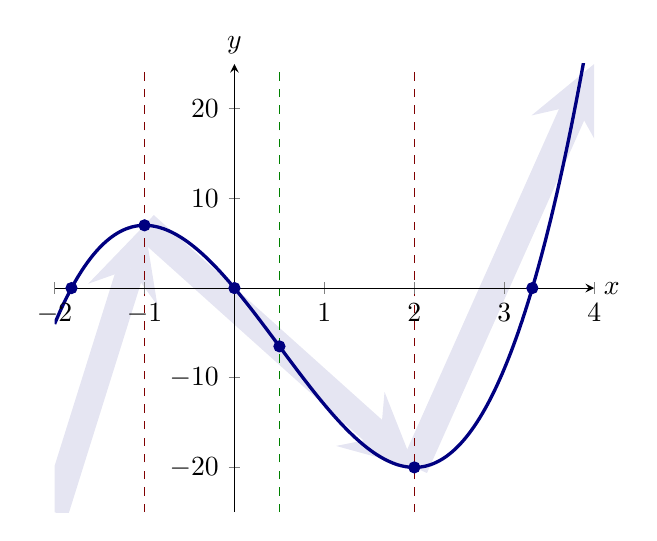
\begin{tikzpicture}
	\begin{axis}[
            axis on top=true,
            domain=-2:4,
            xmin=-2,
            xmax=4,
            ymax=25,
            ymin=-25,
            axis lines =middle, xlabel=$x$, ylabel=$y$,
            every axis y label/.style={at=(current axis.above origin),anchor=south},
            every axis x label/.style={at=(current axis.right of origin),anchor=west}
          ]
          \addplot [->, line width=10, penColor!10!background] plot coordinates {(-2,-25) (-1,7)}; 
          \addplot [->, line width=10, penColor!10!background] plot coordinates {(-1,7) (2,-20)}; 
          \addplot [->, line width=10, penColor!10!background] plot coordinates {(2,-20) (4,25)}; 
          \addplot [dashed, penColor2] plot coordinates {(-1,-25) (-1,25)}; 
          \addplot [dashed, penColor2] plot coordinates {(2,-25) (2,25)}; 
          \addplot [dashed, penColor4] plot coordinates {(1/2,-25) (1/2,25)}; 
          \addplot [color=penColor,fill=penColor,only marks,mark=*] coordinates{(1/2,-6.5)};  %% closed hole
          \addplot [color=penColor,fill=penColor,only marks,mark=*] coordinates{(0,0)};  %% closed hole
          \addplot [color=penColor,fill=penColor,only marks,mark=*] coordinates{(-1,7)};  %% closed hole
          \addplot [color=penColor,fill=penColor,only marks,mark=*] coordinates{(2,-20)};  %% closed hole
          \addplot [color=penColor,fill=penColor,only marks,mark=*] coordinates{(-1.812,0)};  %% closed hole
          \addplot [color=penColor,fill=penColor,only marks,mark=*] coordinates{(3.312,0)};  %% closed hole
          \addplot [very thick, penColor, samples=100, smooth,domain=(-2:4)] {2*x^3-3*x^2-12*x};
        \end{axis}
\end{tikzpicture}
\end{image}

\end{example}

\begin{example}
Sketch the plot of 
\[
f(x) = \begin{cases} xe^x+2 &\text{if $x<0$} \\
x^4-x^2+3 &\text{if $x \geq 0$}.
\end{cases}
\]
NOTE: $\lim_{x \to -\infty}xe^x=0$. You will need this limit when answering some questions below.\\
 Try this on your own first, then either check with a friend, a graphing calculator (like \link[Desmos]{http://www.desmos.com}), or check the online version.


	Since this function is piecewise defined, we will analyze the cases $(-\infty,0)$ and $[0,\infty)$ separately.

	Because $f$ is piecewise defined, and potentially discontinuous at $0$, it is important to understand the behavior of $f$ near $x = 0$.
	
	\[
		\lim_{x \to 0^-} f(x) = \answer[given]{2}
	\]
	
	\[
		\lim_{x \to 0^+} f(x) = \answer[given]{3}
	\]
	
	Moreover, 
	
	\[
	f(0) = \answer[given]{3}
	\]
	
	Record this information on our graph with filled and unfilled circles.

	\begin{image}
\begin{tikzpicture}
	\begin{axis}[
            domain=-5:2,
            xmin=-5,
            xmax=2,
            ymax=5,
            ymin=-1,
            axis lines =middle, xlabel=$x$, ylabel=$y$,
            every axis y label/.style={at=(current axis.above origin),anchor=south},
            every axis x label/.style={at=(current axis.right of origin),anchor=west}
          ]
          \addplot[color=penColor,fill = background, only marks,mark=*] coordinates{(0,2)};
         \addplot[color=penColor,fill=penColor,only marks,mark=*] coordinates{(0,3)};  %% closed hole
        \end{axis}
\end{tikzpicture}
%% \caption{We start by placing the point $(0,0)$.}
%\label{figure:CS1}
\end{image}
	
Which of the following are vertical asymptotes on $(-\infty,0)$?  Select all that apply.

\begin{selectAll}
	\choice{$x=0$}
	\choice{$x=1$}
	\choice{$x=-1$}
	\choice{$x=\sqrt{2}$}
	\choice[correct]{There are no vertical asymptotes}
\end{selectAll}

Which of the following are vertical asymptotes on $(0,\infty)$?  Select all that apply.

\begin{selectAll}
	\choice{$x=0$}
	\choice{$x=1$}
	\choice{$x=-1$}
	\choice{$x=\sqrt{2}$}
	\choice[correct]{There are no vertical asymptotes}
\end{selectAll}


	Which of the following best describes the end behavior of $f$ as $x \to \infty$?
		
		\begin{multipleChoice}
			\choice[correct]{$f$  increases without bound.}
			\choice{$f$ decreases without bound.}
			\choice{$f$ has a horizontal asymptote of $y=2$.}
			\choice{$f$ has some other behavior at $\infty$.}
		\end{multipleChoice}
		
		Which of the following best describes the end behavior of $f$ as $x \to -\infty$?
		
		\begin{multipleChoice}
			\choice{$f$  increases without bound.}
			\choice{$f$ decreases without bound.}
			\choice[correct]{$f$ has a horizontal asymptote of $y = 2$.}
			\choice{$f$ has some other behavior at $\infty$.}
		\end{multipleChoice}

	We mark the location of the horizontal asymptote:
	
	\begin{image}
\begin{tikzpicture}
	\begin{axis}[
             domain=-5:2,
            xmin=-5,
            xmax=2,
            ymax=5,
            ymin=-1,
            axis lines =middle, xlabel=$x$, ylabel=$y$,
            every axis y label/.style={at=(current axis.above origin),anchor=south},
            every axis x label/.style={at=(current axis.right of origin),anchor=west}
          ]
         \addplot[color=penColor,fill = background, only marks,mark=*] coordinates{(0,2)};
         \addplot[color=penColor,fill=penColor,only marks,mark=*] coordinates{(0,3)};  %% closed hole
         \addplot [dashed, penColor2] plot coordinates {(-5,2) (0,2)}; 
        \end{axis}
\end{tikzpicture}
%\caption{Now we add the critical points $x=-1$ and $x=2$.}
%\label{figure:CS2}
\end{image}
	
		The derivative of $f$ on $(-\infty, 0)$ is
		\[
		f'(x)= \answer[given]{xe^x+e^x}=e^x(\answer[given]{x+1})
		\]
				
		The derivative of $f$ on $(0, \infty)$ is
		\[
		f'(x)= \answer[given]{4x^3-2x}=4x(\answer[given]{x^2-\frac{1}{2}})
		\]
		

The critical points are where $f'(x) = 0$ or does not exist.  $0$ is a critical point, since we have already seen it is a point of discontinuity for $f$, and thus $f'(0)$ does not exist there.

On $(-\infty, 0)$, $f$ has a critical point at $x = \answer[given]{-1}$ 

On $(0,\infty)$, $f$ has a critical point at $x = \answer[given]{\frac{1}{\sqrt{2}}}$

Mark the critical points $x=-1$ and $x=\frac{1}{\sqrt{2}}$ on your plot. %%BADBAD either or answer would be nice
\begin{image}
\begin{tikzpicture}
	\begin{axis}[
             domain=-5:2,
            xmin=-5,
            xmax=2,
            ymax=5,
            ymin=-1,
            axis lines =middle, xlabel=$x$, ylabel=$y$,
            every axis y label/.style={at=(current axis.above origin),anchor=south},
            every axis x label/.style={at=(current axis.right of origin),anchor=west}
          ]
         \addplot[color=penColor,fill = background, only marks,mark=*] coordinates{(0,2)};
         \addplot[color=penColor,fill=penColor,only marks,mark=*] coordinates{(0,3)};  %% closed hole
         \addplot [dashed, penColor2] plot coordinates {(-5,2) (0,2)}; 
         \addplot [dashed, penColor2] plot coordinates {(-1,-1) (-1,5)}; 
         \addplot [dashed, penColor2] plot coordinates {(0.70710678118,-1) (0.70710678118,5)}; 
        \end{axis}
\end{tikzpicture}
%\caption{Now we add the critical points $x=-1$ and $x=2$.}
%\label{figure:CS2}
\end{image}

Using the first derivative, we can see that 

On $(-\infty, -1)$, $f'(x)=e^x(x+1)$ and has the same sign as the factor $(x+1)$, which is negative. Therefore, $f$ is \wordChoice{ \choice{increasing} \choice[correct]{decreasing}} on $(-\infty, -1)$.

On $(-1, 0)$, $f'(x)$ has the same sign as the factor $(x+1)$, which is positive. Therefore, \wordChoice{ \choice[correct]{increasing} \choice{decreasing}} on $(-1, 0)$.

On $(0, \frac{1}{\sqrt{2}})$, since $f'(\frac{1}{4})= \frac{1}{16}-\frac{1}{2}<0$, $f$ is \wordChoice{ \choice{increasing} \choice[correct]{decreasing}}.

On $(\frac{1}{\sqrt{2}}, \infty)$, since $f'(1)= 4(1-\frac{1}{2})>0$,  $f$ is \wordChoice{ \choice[correct]{increasing} \choice{decreasing}}.

\begin{image}
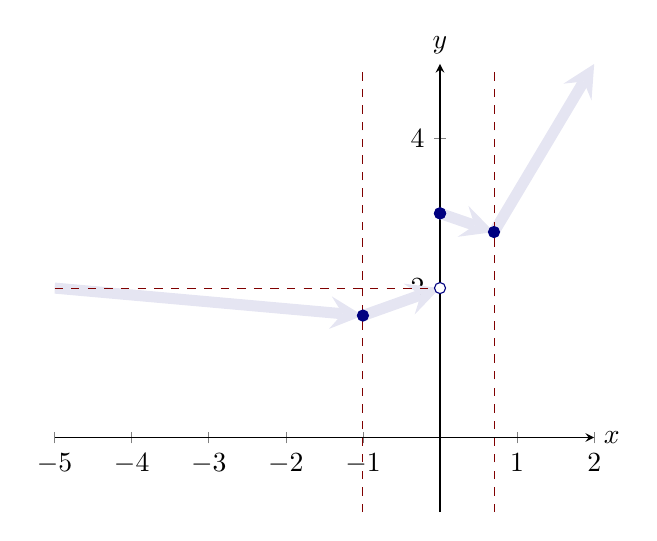
\begin{tikzpicture}
	\begin{axis}[
             domain=-5:2,
            xmin=-5,
            xmax=2,
            ymax=5,
            ymin=-1,
            axis lines =middle, xlabel=$x$, ylabel=$y$,
            every axis y label/.style={at=(current axis.above origin),anchor=south},
            every axis x label/.style={at=(current axis.right of origin),anchor=west}
          ]
           \addplot [->, line width=4, penColor!10!background] plot coordinates {(-5,2) (-1,1.632)}; 
            \addplot [->, line width=4, penColor!10!background] plot coordinates {(-1,1.632) (0,2)}; 
             \addplot [->, line width=4, penColor!10!background] plot coordinates {(0,3) (.7,2.75)}; 
              \addplot [->, line width=4, penColor!10!background] plot coordinates {(.7,2.75) (2,5)}; 
         \addplot[color=penColor,fill = background, only marks,mark=*] coordinates{(0,2)};
         \addplot[color=penColor,fill=penColor,only marks,mark=*] coordinates{(0,3)};  %% closed hole
\addplot[color=penColor,fill=penColor,only marks,mark=*] coordinates{(-1,1.632)};
\addplot[color=penColor,fill=penColor,only marks,mark=*] coordinates{(0.7,2.75)};
\addplot[color=penColor,fill=penColor,only marks,mark=*] coordinates{(0,3)};
         \addplot [dashed, penColor2] plot coordinates {(-5,2) (0,2)}; 
         \addplot [dashed, penColor2] plot coordinates {(-1,-1) (-1,5)}; 
         \addplot [dashed, penColor2] plot coordinates {(0.70710678118,-1) (0.70710678118,5)}; 
        \end{axis}
\end{tikzpicture}
%\caption{Now we add the critical points $x=-1$ and $x=2$.}
%\label{figure:CS2}
\end{image}
The second derivative of $f$ on $(-\infty, 0)$ is 
		\[
		f''(x)= \answer[given]{xe^x+2e^x}=e^x(\answer[given]{x+2})
		\]

The second derivative of $f$ on $(0, \infty)$ is 
		\[
		f''(x)= \answer[given]{12x^2-2}=12(\answer[given]{x^2-\frac{1}{6}})
		\]
The candidates for the inflection points are where $f''(x) = 0$.

On $(-\infty, 0)$, $f''$ has one zero, namely $x = \answer[given]{-2}$.  The sign of $f''$ changes from \wordChoice{\choice{positive to negative} \choice[correct]{negative to positive}]} through this point.

On $(0, \infty)$, $f''$ has one zero, namely $x = \answer[given]{\frac{1}{\sqrt{6}}}$. The sign of $f''$ changes from \wordChoice{\choice{positive to negative} \choice[correct]{negative to positive}]} through this point.

\begin{image}
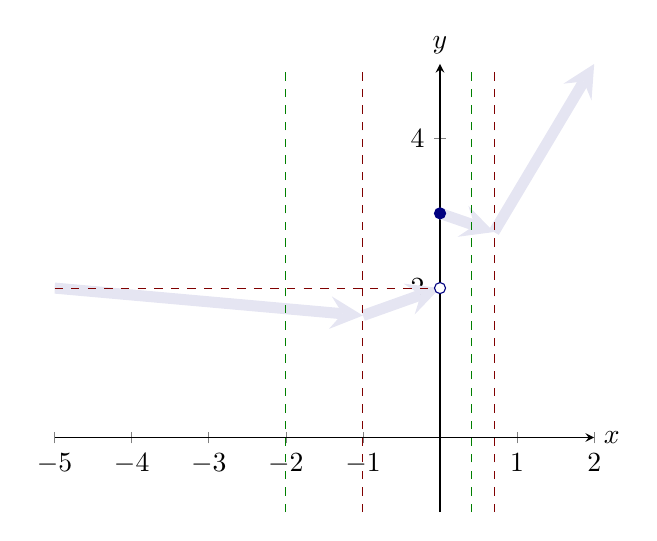
\begin{tikzpicture}
	\begin{axis}[
             domain=-5:2,
            xmin=-5,
            xmax=2,
            ymax=5,
            ymin=-1,
            axis lines =middle, xlabel=$x$, ylabel=$y$,
            every axis y label/.style={at=(current axis.above origin),anchor=south},
            every axis x label/.style={at=(current axis.right of origin),anchor=west}
          ]
           \addplot [->, line width=4, penColor!10!background] plot coordinates {(-5,2) (-1,1.632)}; 
            \addplot [->, line width=4, penColor!10!background] plot coordinates {(-1,1.632) (0,2)}; 
             \addplot [->, line width=4, penColor!10!background] plot coordinates {(0,3) (.7,2.75)}; 
              \addplot [->, line width=4, penColor!10!background] plot coordinates {(.7,2.75) (2,5)}; 
         \addplot[color=penColor,fill = background, only marks,mark=*] coordinates{(0,2)};
         \addplot[color=penColor,fill=penColor,only marks,mark=*] coordinates{(0,3)};  %% closed hole
         \addplot [dashed, penColor2] plot coordinates {(-5,2) (0,2)}; 
         \addplot [dashed, penColor2] plot coordinates {(-1,-1) (-1,5)}; 
         \addplot [dashed, penColor2] plot coordinates {(0.70710678118,-1) (0.70710678118,5)}; 
         \addplot [dashed, penColor4] plot coordinates {(-2,-1) (-2,5)}; 
         \addplot [dashed, penColor4] plot coordinates {(0.40824829046,-1) (0.40824829046,5)}; 
        \end{axis}
\end{tikzpicture}
%\label{figure:CS2}
\end{image}

Since all of this behavior as described above occurs on the interval
$[-5,2]$, we now have a complete sketch of $y=f(x)$ on this interval,
see the figure below.
\begin{image}
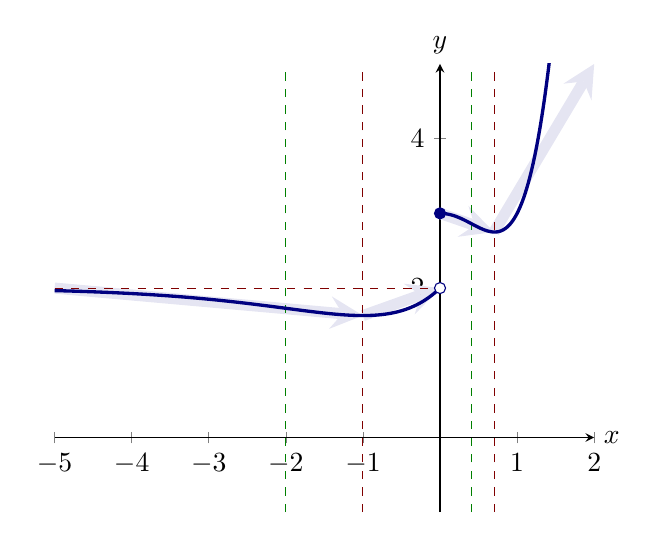
\begin{tikzpicture}
	\begin{axis}[
             domain=-5:2,
            xmin=-5,
            xmax=2,
            ymax=5,
            ymin=-1,
            axis lines =middle, xlabel=$x$, ylabel=$y$,
            every axis y label/.style={at=(current axis.above origin),anchor=south},
            every axis x label/.style={at=(current axis.right of origin),anchor=west}
          ]
           \addplot [->, line width=4, penColor!10!background] plot coordinates {(-5,2) (-1,1.632)}; 
            \addplot [->, line width=4, penColor!10!background] plot coordinates {(-1,1.632) (0,2)}; 
             \addplot [->, line width=4, penColor!10!background] plot coordinates {(0,3) (.7,2.75)}; 
              \addplot [->, line width=4, penColor!10!background] plot coordinates {(.7,2.75) (2,5)}; 
         \addplot[color=penColor,fill = background, only marks,mark=*] coordinates{(0,2)};
         \addplot[color=penColor,fill=penColor,only marks,mark=*] coordinates{(0,3)};  %% closed hole
         \addplot [dashed, penColor2] plot coordinates {(-5,2) (0,2)}; 
         \addplot [dashed, penColor2] plot coordinates {(-1,-1) (-1,5)}; 
         \addplot [dashed, penColor2] plot coordinates {(0.70710678118,-1) (0.70710678118,5)}; 
         \addplot [dashed, penColor4] plot coordinates {(-2,-1) (-2,5)}; 
         \addplot [dashed, penColor4] plot coordinates {(0.40824829046,-1) (0.40824829046,5)}; 
          \addplot [very thick, penColor, samples=100, smooth,domain=(-5:0)] {x*e^x+2};
          \addplot [very thick, penColor, samples=100, smooth,domain=(0:2)] {x^4-x^2+3};
        \end{axis}
\end{tikzpicture}
%\label{figure:CS2}
\end{image}
\end{example}
\end{document}
